%% \author{
%%         Vitaly Surazhsky \\
%%                 Department of Computer Science\\
%%         Technion---Israel Institute of Technology\\
%%         Technion City, Haifa 32000, \underline{Israel}
%%             \and
%%         Yossi Gil\\
%%         Department of Computer Science\\
%%         Technion---Israel Institute of Technology\\
%%         Technion City, Haifa 32000, \underline{Israel}
%% }
\date{\vspace{-5ex}}
%% \date{\today}

\documentclass[9pt]{article}
\usepackage{geometry}
\geometry{legalpaper, portrait, margin=1.5in}


\usepackage{graphicx}
\usepackage{titling}

\title{FOSSEE - Promoting Free and Open Source Software in Education}{\vspace{-5ex}}


\begin{document}
\setlength{\droptitle}{-3cm}    %remove extra title vertical spacing

\maketitle

The aim of the FOSSEE project (http://fossee.in) is to eliminate the
use of proprietary/commercial software packages in Science and
Engineering Education across India and replace them with Free and Open
Source Software (FOSS). The shift to FOSS packages will help
educational institutions monetarily. \\

\begin{figure}[ht]
\centering
\fboxsep=0mm%padding thickness
\fboxrule=1pt%border thickness   
{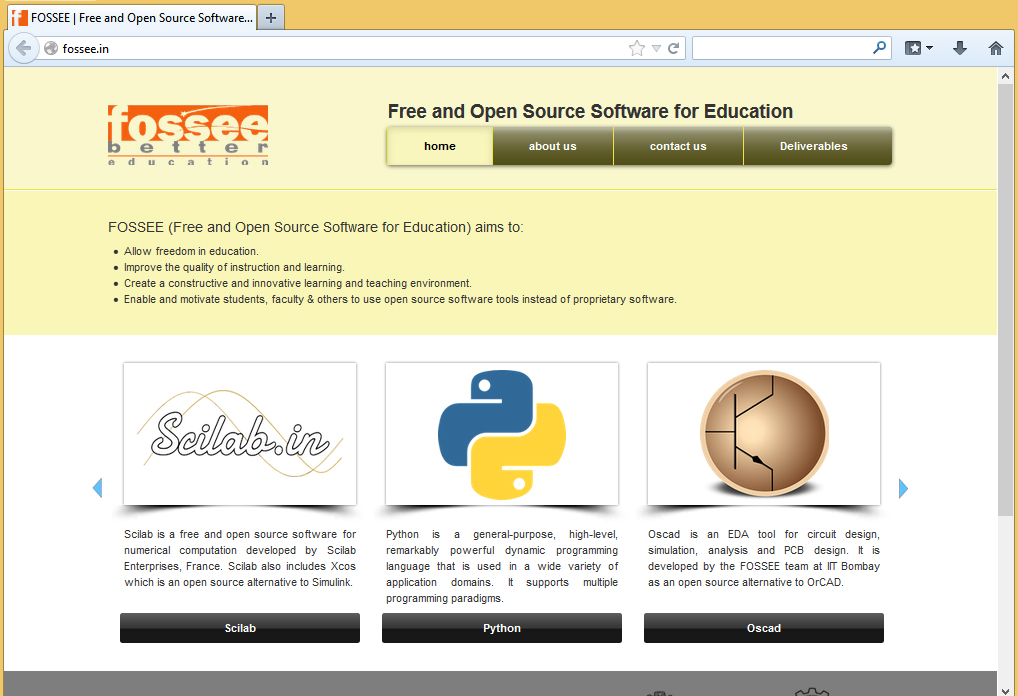
\includegraphics[width=1\columnwidth]{fossee-site.png}}
\caption{http://fossee.in}\label{fossee}
\end{figure}

Two of the flagship activities promoted by the FOSSEE team are
{\bf{Textbook Companion}} (TBC) and {\bf{Lab Migration.}} \\

One of the major shortcomings of FOSS tools is the lack of
documentation. FOSSEE addresses this important issue by promoting
Textbook Companion activity. {\bf{Textbook Companion}} activity
creates code for solved examples of standard textbooks using FOSS. It
is available online for free download and use. It is done by students
and the faculty of colleges from different parts of India. \\

As long as a college uses proprietary tools as part of their lab
curriculum, we cannot eliminate the use of commercial software. To
address this issue, we have started the {\bf{Lab Migration}} activity
that aims to migrate college labs using proprietary software to a FOSS
only lab. The FOSS code created by a student/teacher is released in
open source code for public use. \\

Students and faculty involved in both the above mentioned activities
are given honorarium for their efforts. \\

Various other FOSSEE activities are as follows:

\begin{itemize}
\item{{\bf{SELF Workshops}}: are Spoken Tutorial based Education and Learning
through Free FOSS study workshops. These workshops have been conducted
in different parts of India. During the last one year, a total of
about 450 Scilab, 240 Python and 8 OpenFOAM, SELF workshops have been
conducted in this manner, training about 22,000 students and faculty
members.}
\item{{\bf{Course Conversion}}: The course conversion effort aims to provide
the necessary help to teach a course using Scilab. Five courses have
been converted using Scilab.}
\item{{\bf{Hardware Interface}}: FOSSEE has come up with Scilab based data
acquisition systems using COMEDI (COntrol and MEasurement Device
Interface with drivers for more than 400 A/D cards and digital I/O
cards), Xcos (block oriented simulation tool) and HART (hardware
access real time toolbox).}
\item{{\bf{FOSS on Aakash}}: The FOSSEE team helped port C, C++, Python,
Scilab and Oscad onto the Aakash tablet.}
\end{itemize} 

Currently, FOSSEE team promotes the following software extensively: \\

{\bf{Scilab}} is a free and open source software for numerical
computation developed by Scilab Enterprises, France. It is a FOSS
alternative to MATLAB.  It also includes Xcos which is an open source
alternative to Simulink. The Scilab team have successfully created
more than 275 Textbook Companions and ported 12 labs through the Lab
Migration activity till date. To increase ease of executing Textbook
Companion code online, FOSSEE has ported TBC on GARUDA cloud
(http://scilab.in/scilab-on-cloud). Please visit http://scilab.in for
more details. \\

{\bf{Python}} is a general-purpose interpreted, high-level,
object-oriented programming language that is used in a wide variety of
application domains.The Python team promotes the use of the language
through Python Textbook Companion. Under Python Textbook Companion, 53
textbook companions have been completed. For more information visit
http://python.fossee.in/ \\

{\bf{Oscad}} is developed by the FOSSEE team at IIT Bombay it is an
EDA tool for circuit design, simulation, analysis and PCB design. Free
tutorials of Oscad are available at
http://oscad.in/resources/tutorials. \\

{\bf{COIN-OR}} or {\bf{CO}}mputational {\bf{IN}}frastructure for
{\bf{O}}perations {\bf{R}}esearch is a project to build and support an
open-source software for operations research and its
applications. {\bf{Simpy}} (Simulation in Python) is an open source,
Python-based, discrete-event simulation software.  OR Tools at FOSSEE
is promoting COIN-OR, Simpy and other FOSS by developing tutorials,
textbook companions and software interfaces in Scilab and Python. For
more details please visit http://or.fossee.in \\

{\bf{OpenFOAM}} is a free, open source CFD software package developed
by OpenCFD Ltd and distributed by the OpenFOAM Foundation. Tutorials
in the form of web-casts, for self learning OpenFOAM have been
developed by our team. These are available free of cost at
http://cfd.fossee.in. \\

The FOSSEE team is dedicated in promoting FOSS tools in educational
institutions across India. We invite institutions to join us in making
this project a success for years to come.


%% \bibliographystyle{abbrv}
%% \bibliography{simple}

\end{document}
This is never printed
